\section{Ejemplo 1}

    \lipsum[1]
    
    \begin{figure}[h]
    	\centering
    	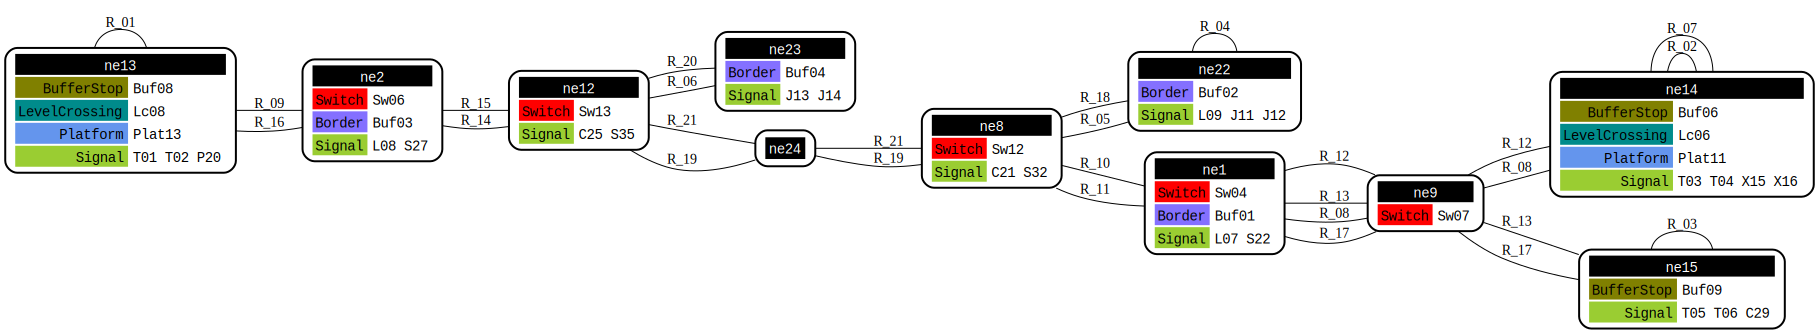
\includegraphics[width=1\textwidth]{Figuras/Graph_1}
    	\centering\caption{XXXX}
    	%\label{fig:LC_P2}
    \end{figure}
    
    \lipsum[1]

    \begin{figure}[h]
        \centering
        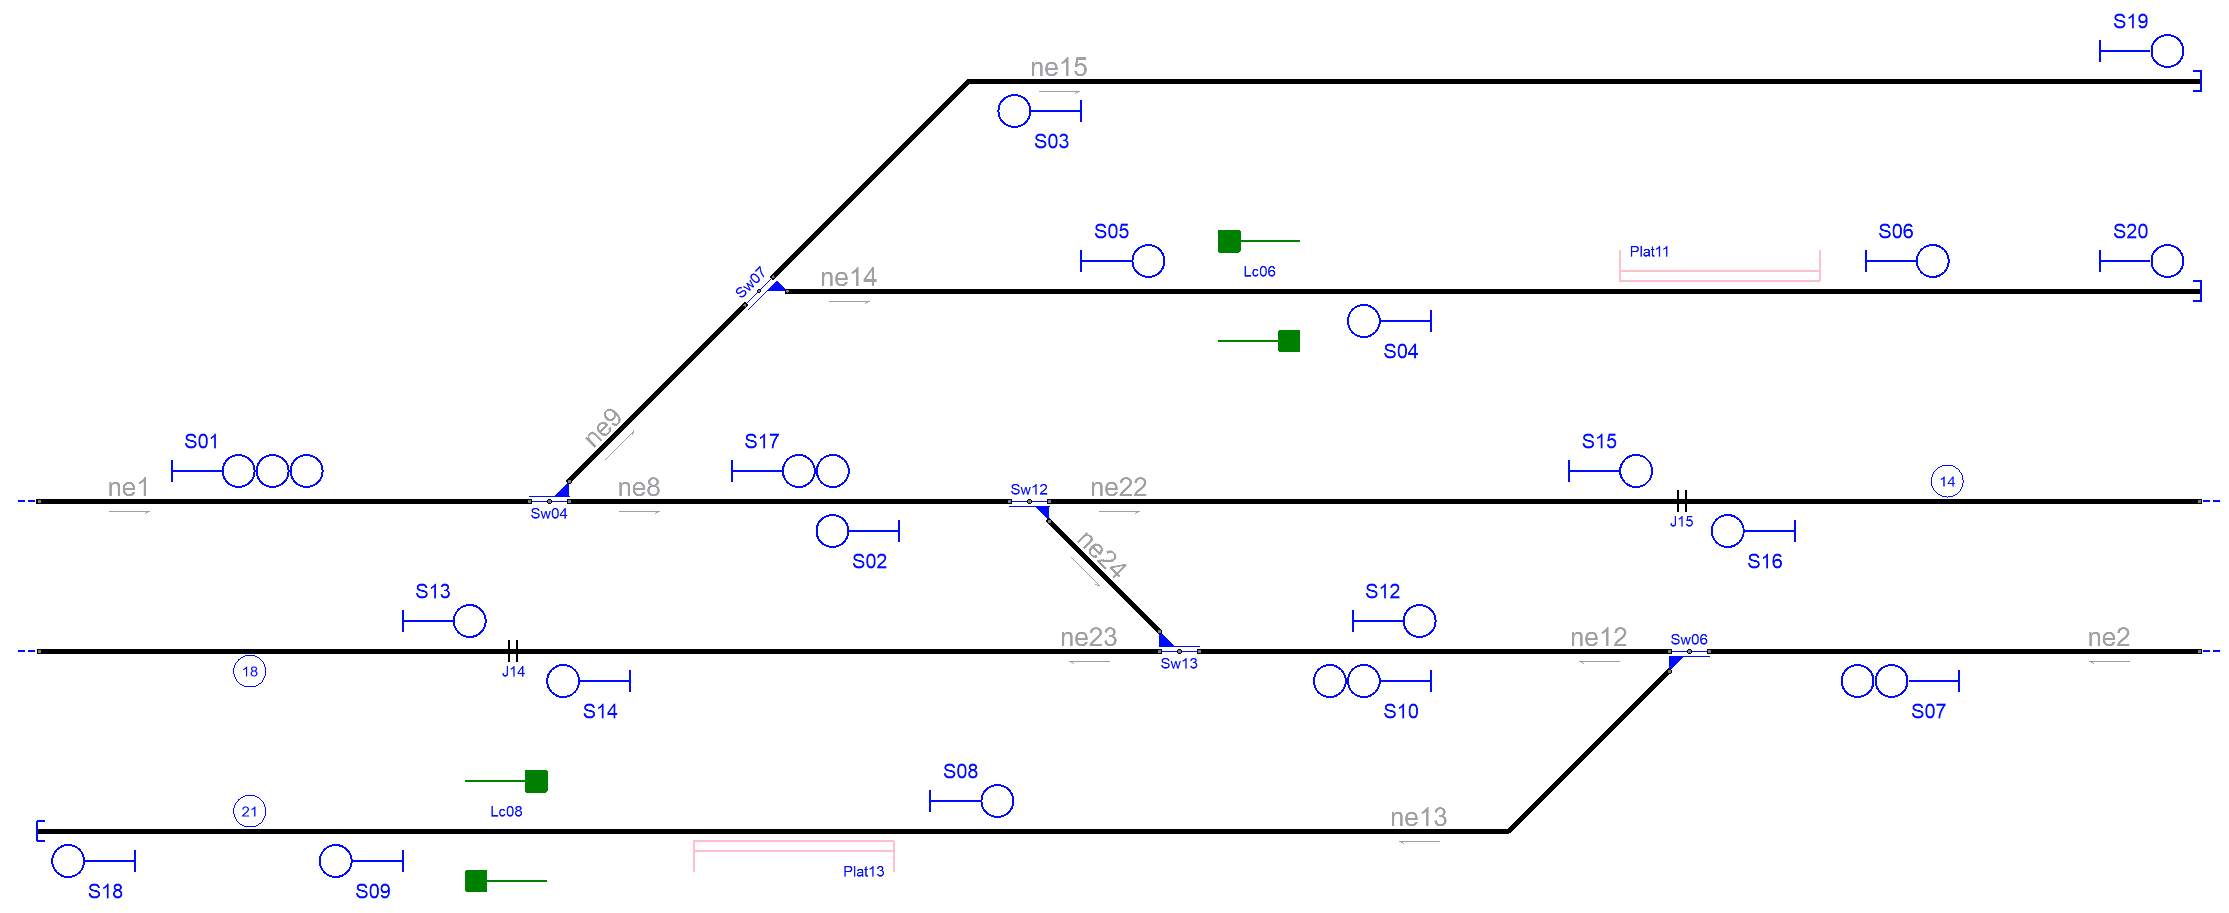
\includegraphics[width=1\textwidth]{resultados-obtenidos/ejemplo1/images/1_original.png}
        \centering\caption{Señalamiento original del ejemplo 1.}
        %\label{fig:LC_P2}
    \end{figure}

    \begin{figure}[h]
        \centering
        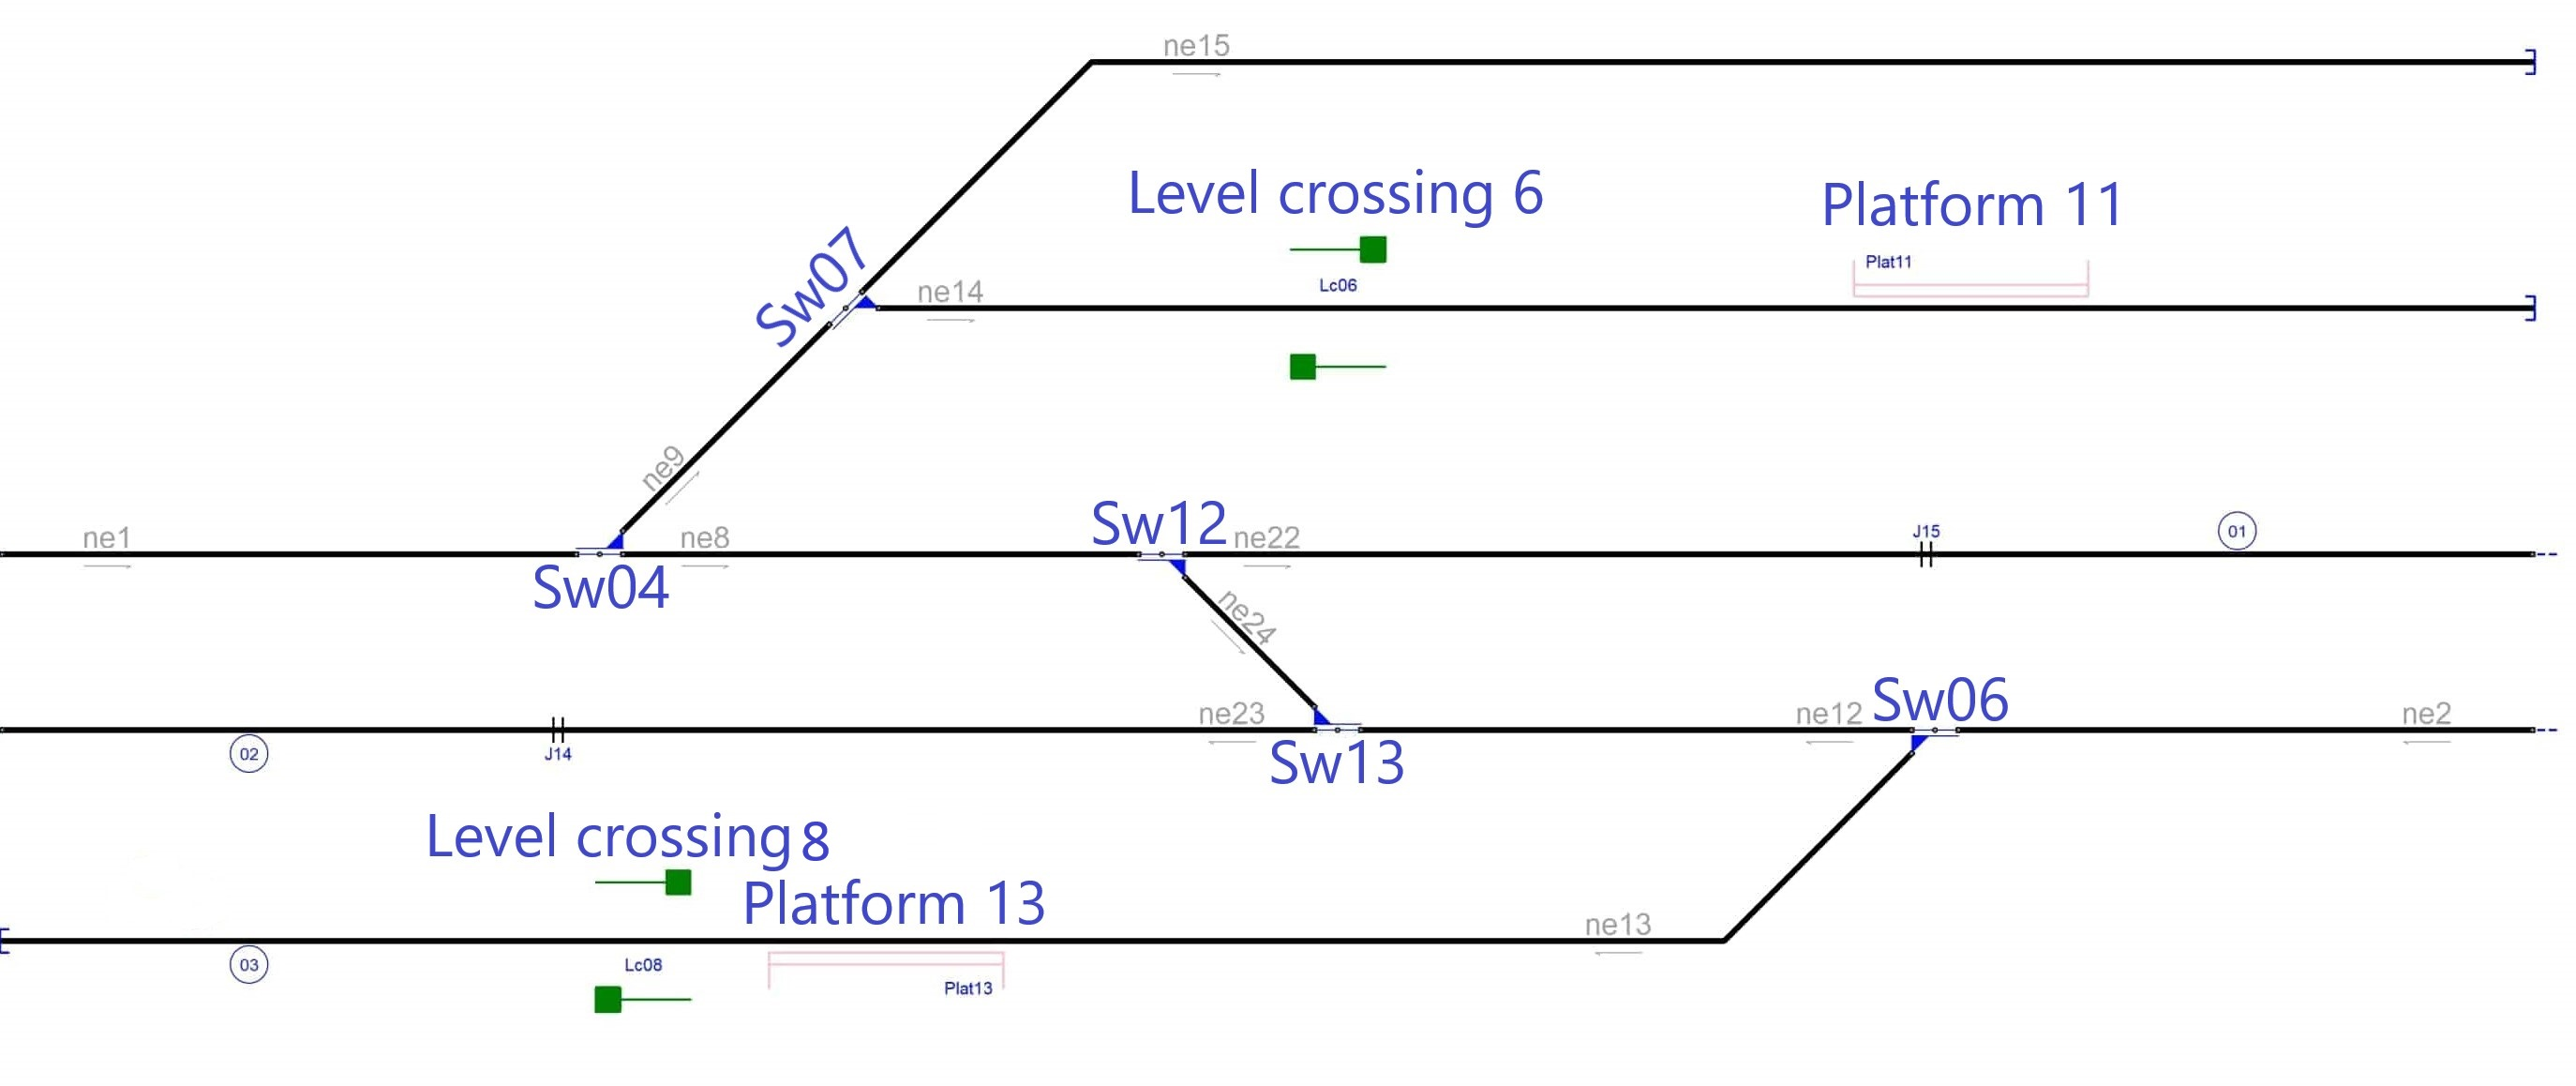
\includegraphics[width=1\textwidth]{resultados-obtenidos/ejemplo1/images/1_empty.png}
        \centering\caption{Topología ferroviaria del ejemplo 1 sin señalamiento.}
        %\label{fig:LC_P2}
    \end{figure}

    \begin{figure}[h]
        \centering
        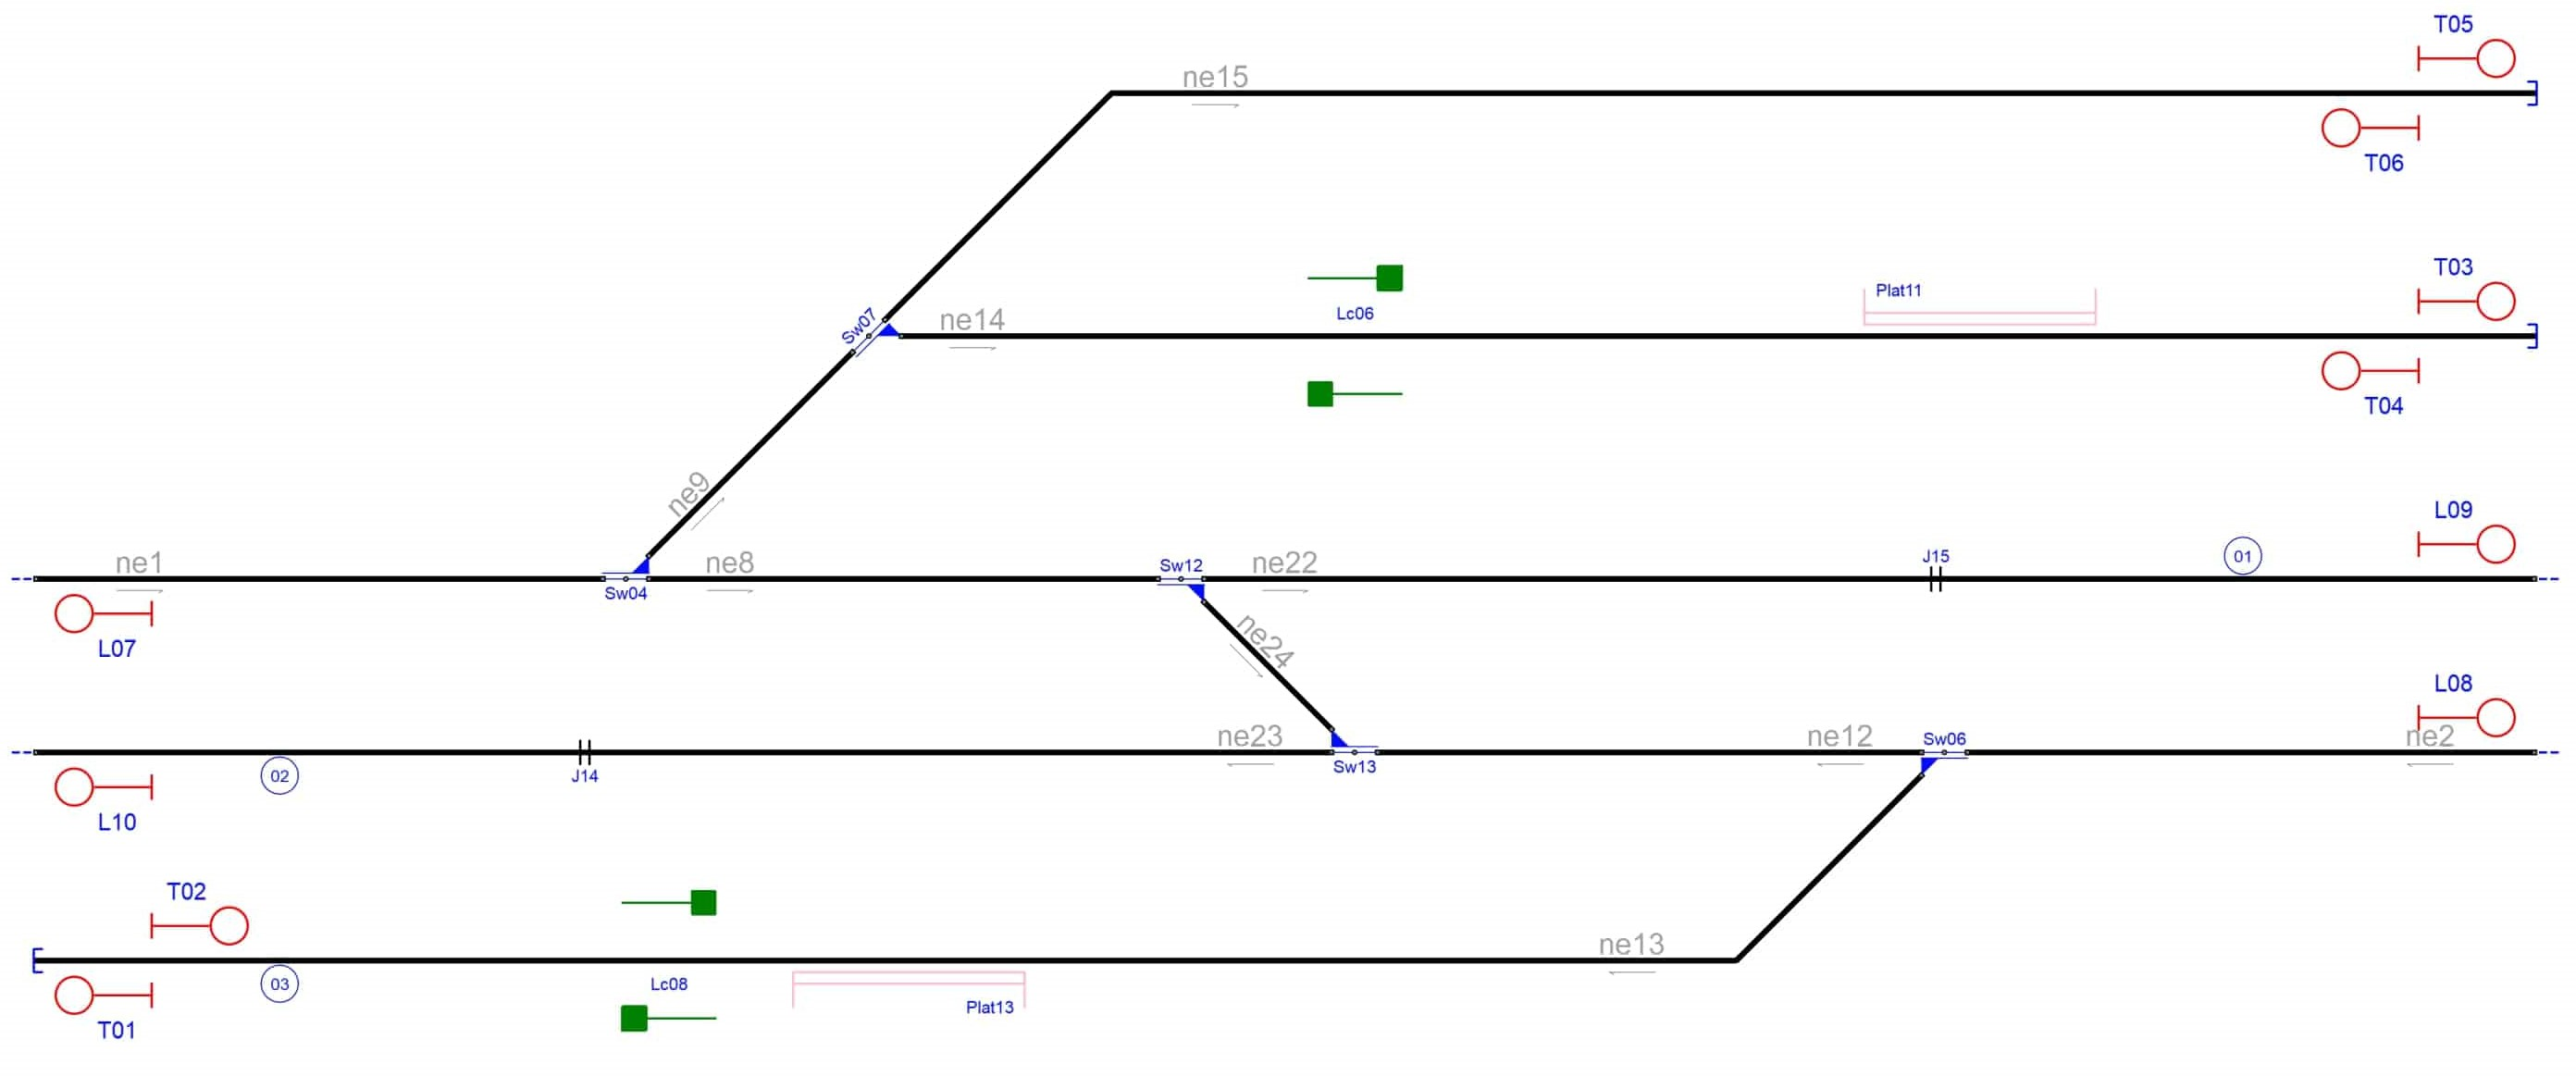
\includegraphics[width=1\textwidth]{resultados-obtenidos/ejemplo1/images/1_step1.png}
        \centering\caption{Señalamiento generado por el RNA para proteger el fín de vía.}
        %\label{fig:LC_P2}
    \end{figure}

    \begin{figure}[h]
        \centering
        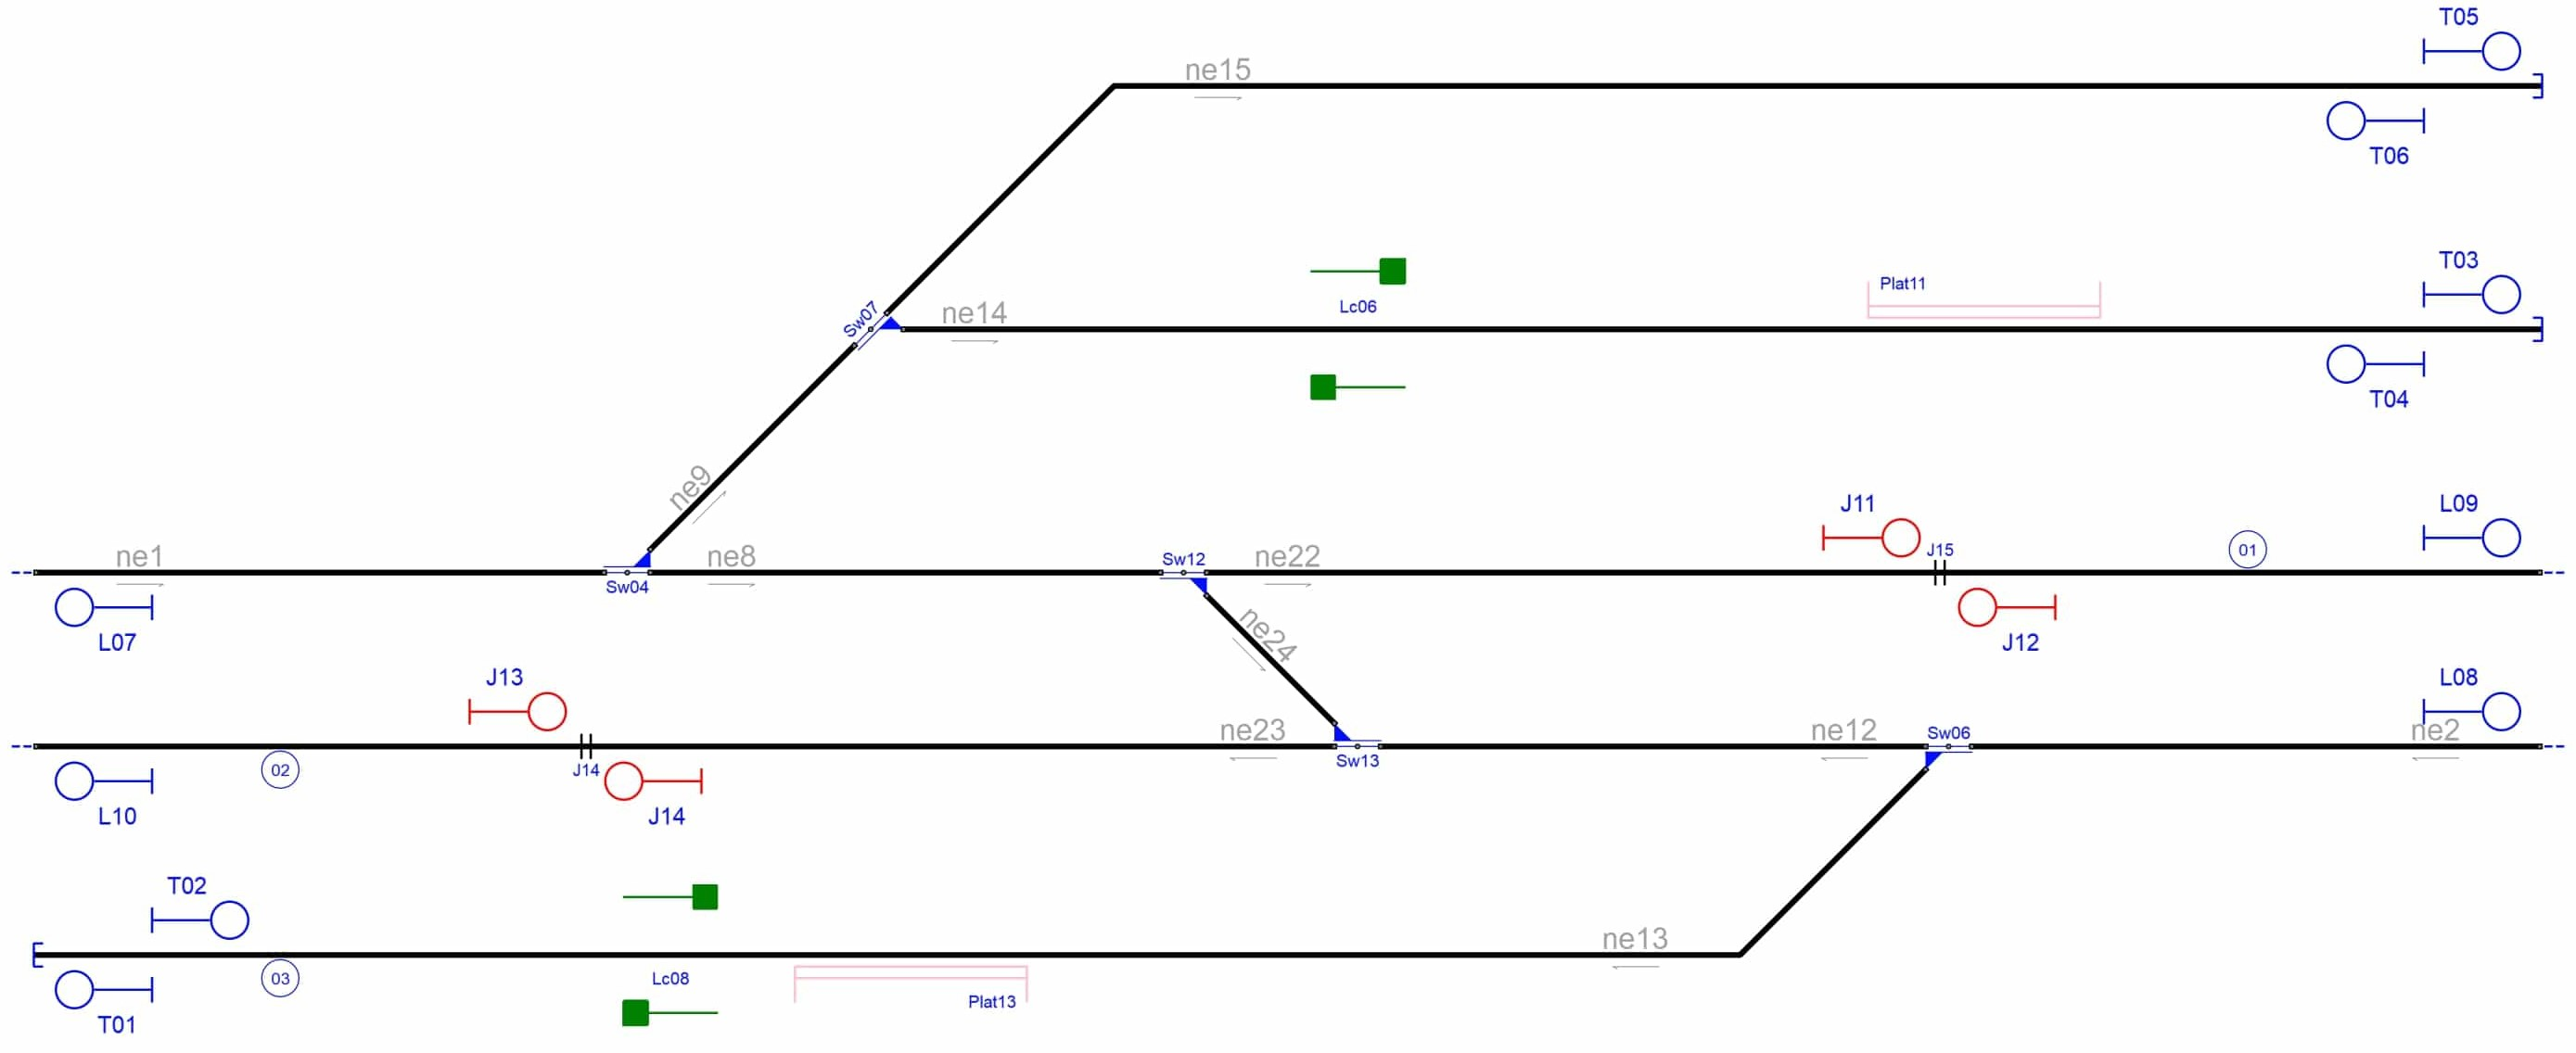
\includegraphics[width=1\textwidth]{resultados-obtenidos/ejemplo1/images/1_step2.png}
        \centering\caption{Señalamiento generado por el RNA para proteger las junturas.}
        %\label{fig:LC_P2}
    \end{figure}

    \begin{figure}[h]
        \centering
        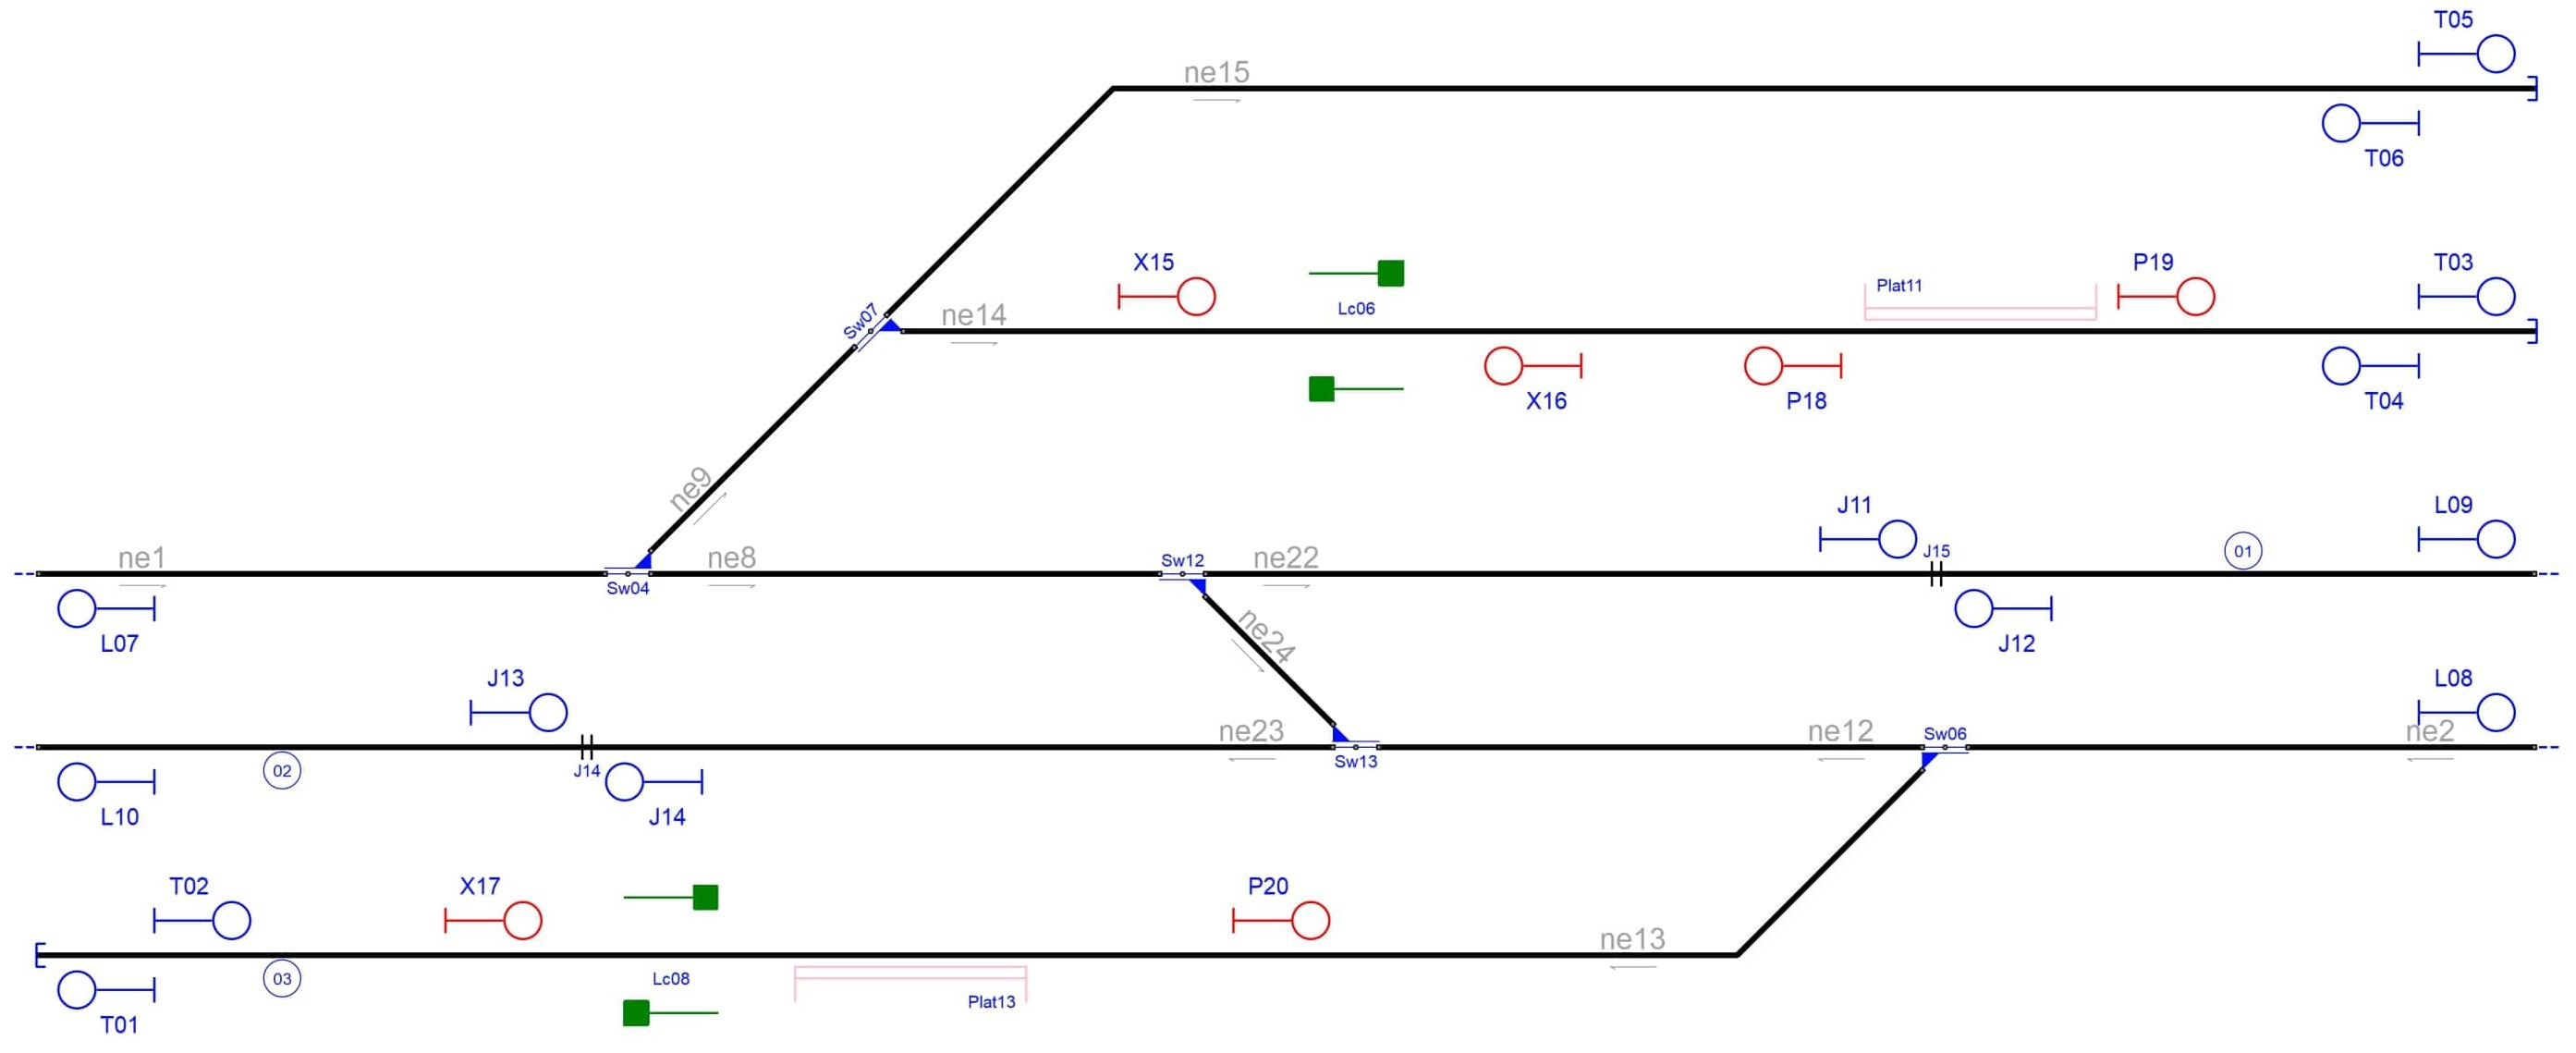
\includegraphics[width=1\textwidth]{resultados-obtenidos/ejemplo1/images/1_step3.png}
        \centering\caption{Señalamiento generado por el RNA para proteger plataformas y cruces de vía.}
        %\label{fig:LC_P2}
    \end{figure}

    \begin{figure}[h]
        \centering
        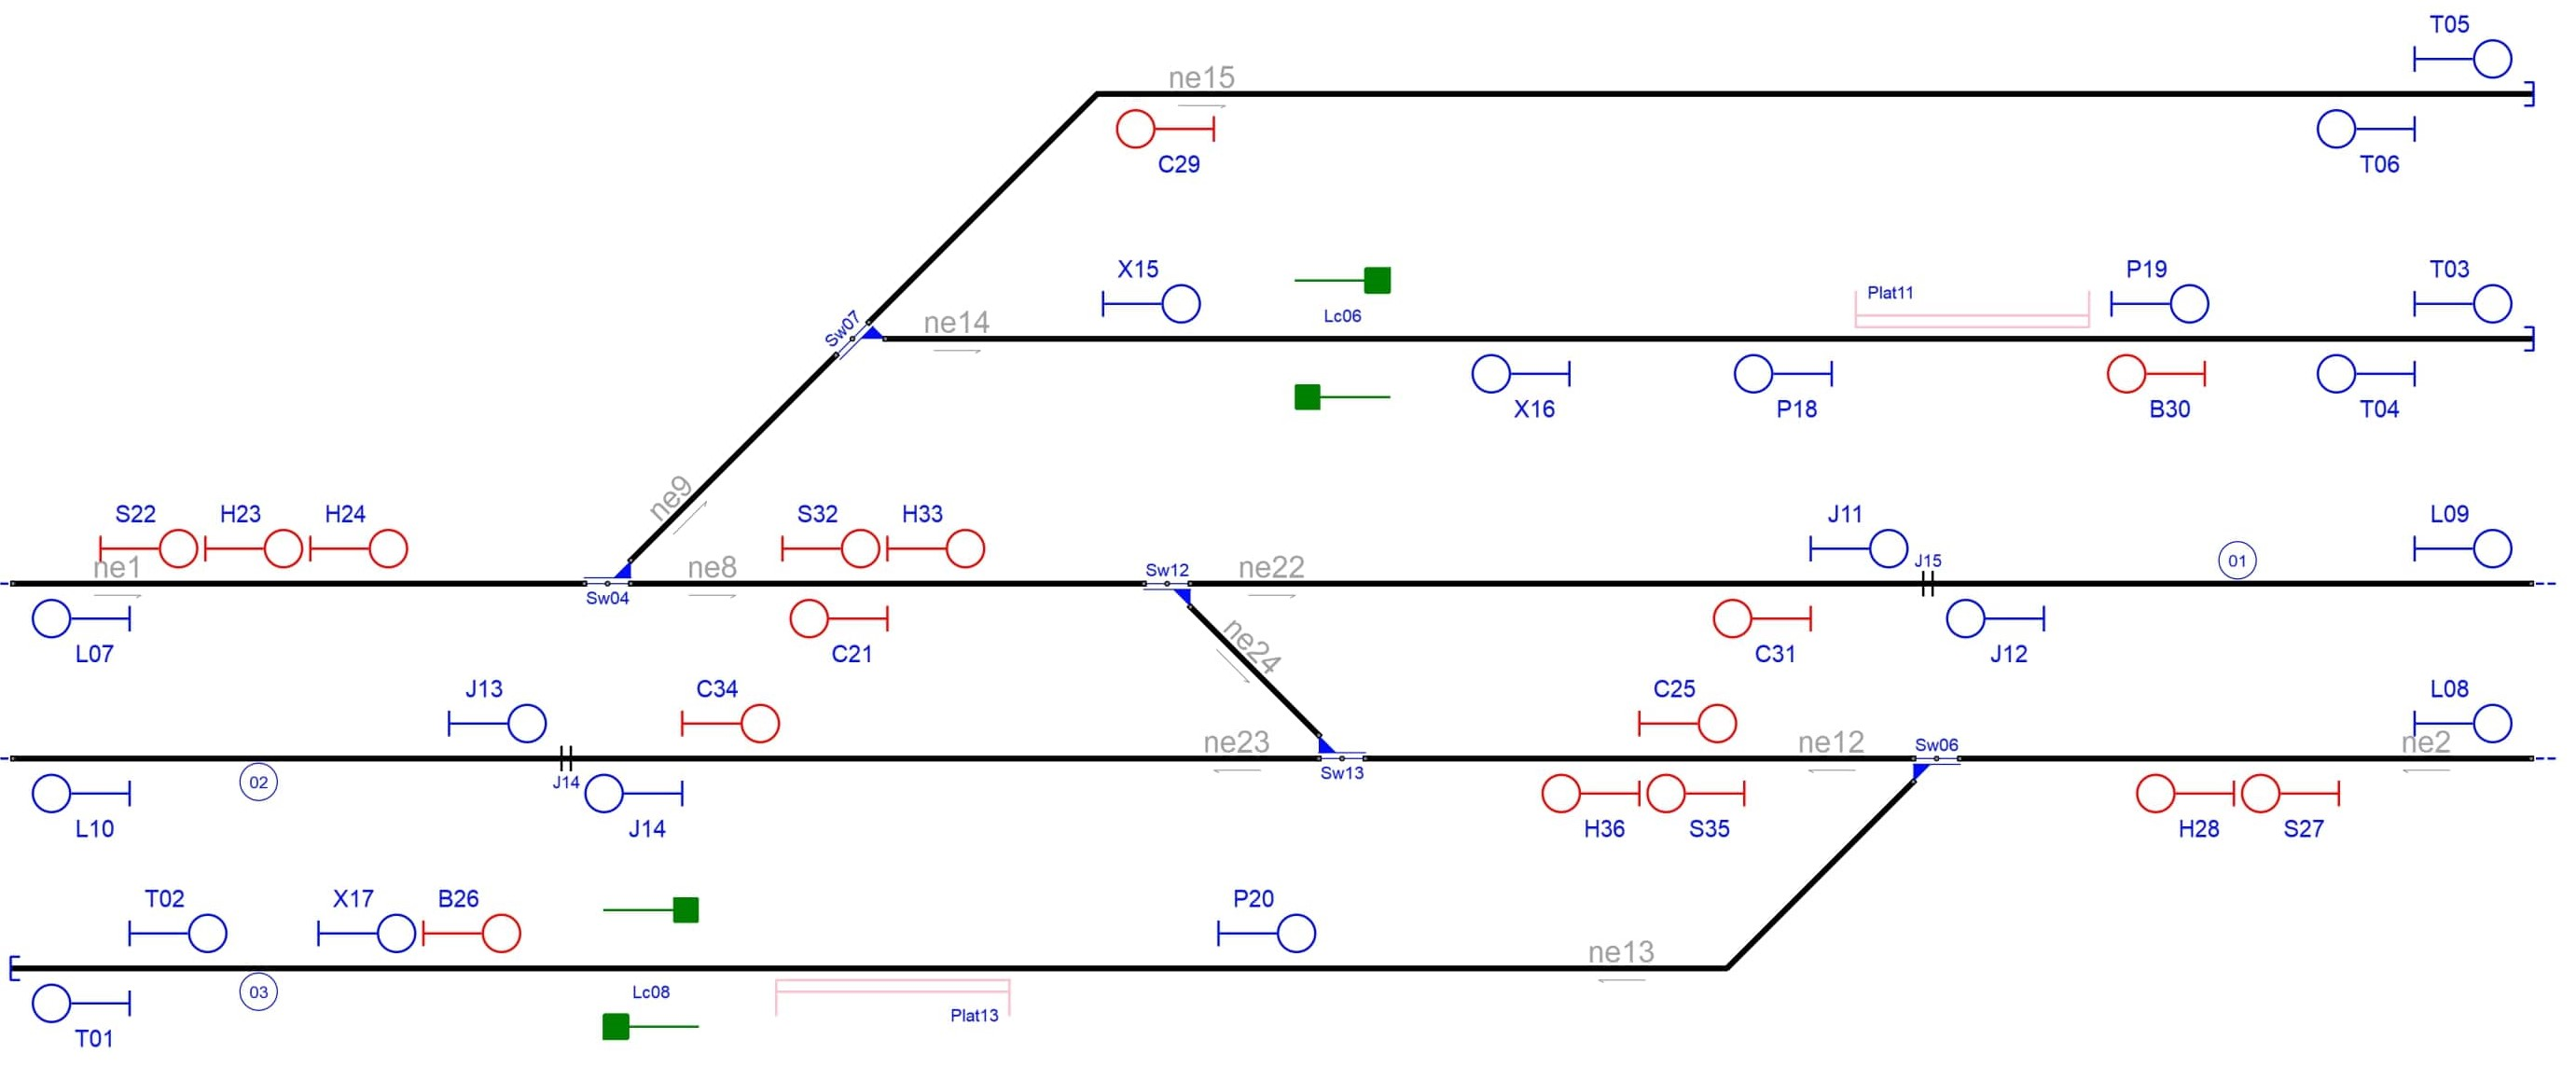
\includegraphics[width=1\textwidth]{resultados-obtenidos/ejemplo1/images/1_step4.png}
        \centering\caption{Señalamiento generado por el RNA para proteger las máquinas de cambios.}
        %\label{fig:LC_P2}
    \end{figure}

    \begin{figure}[h]
        \centering
        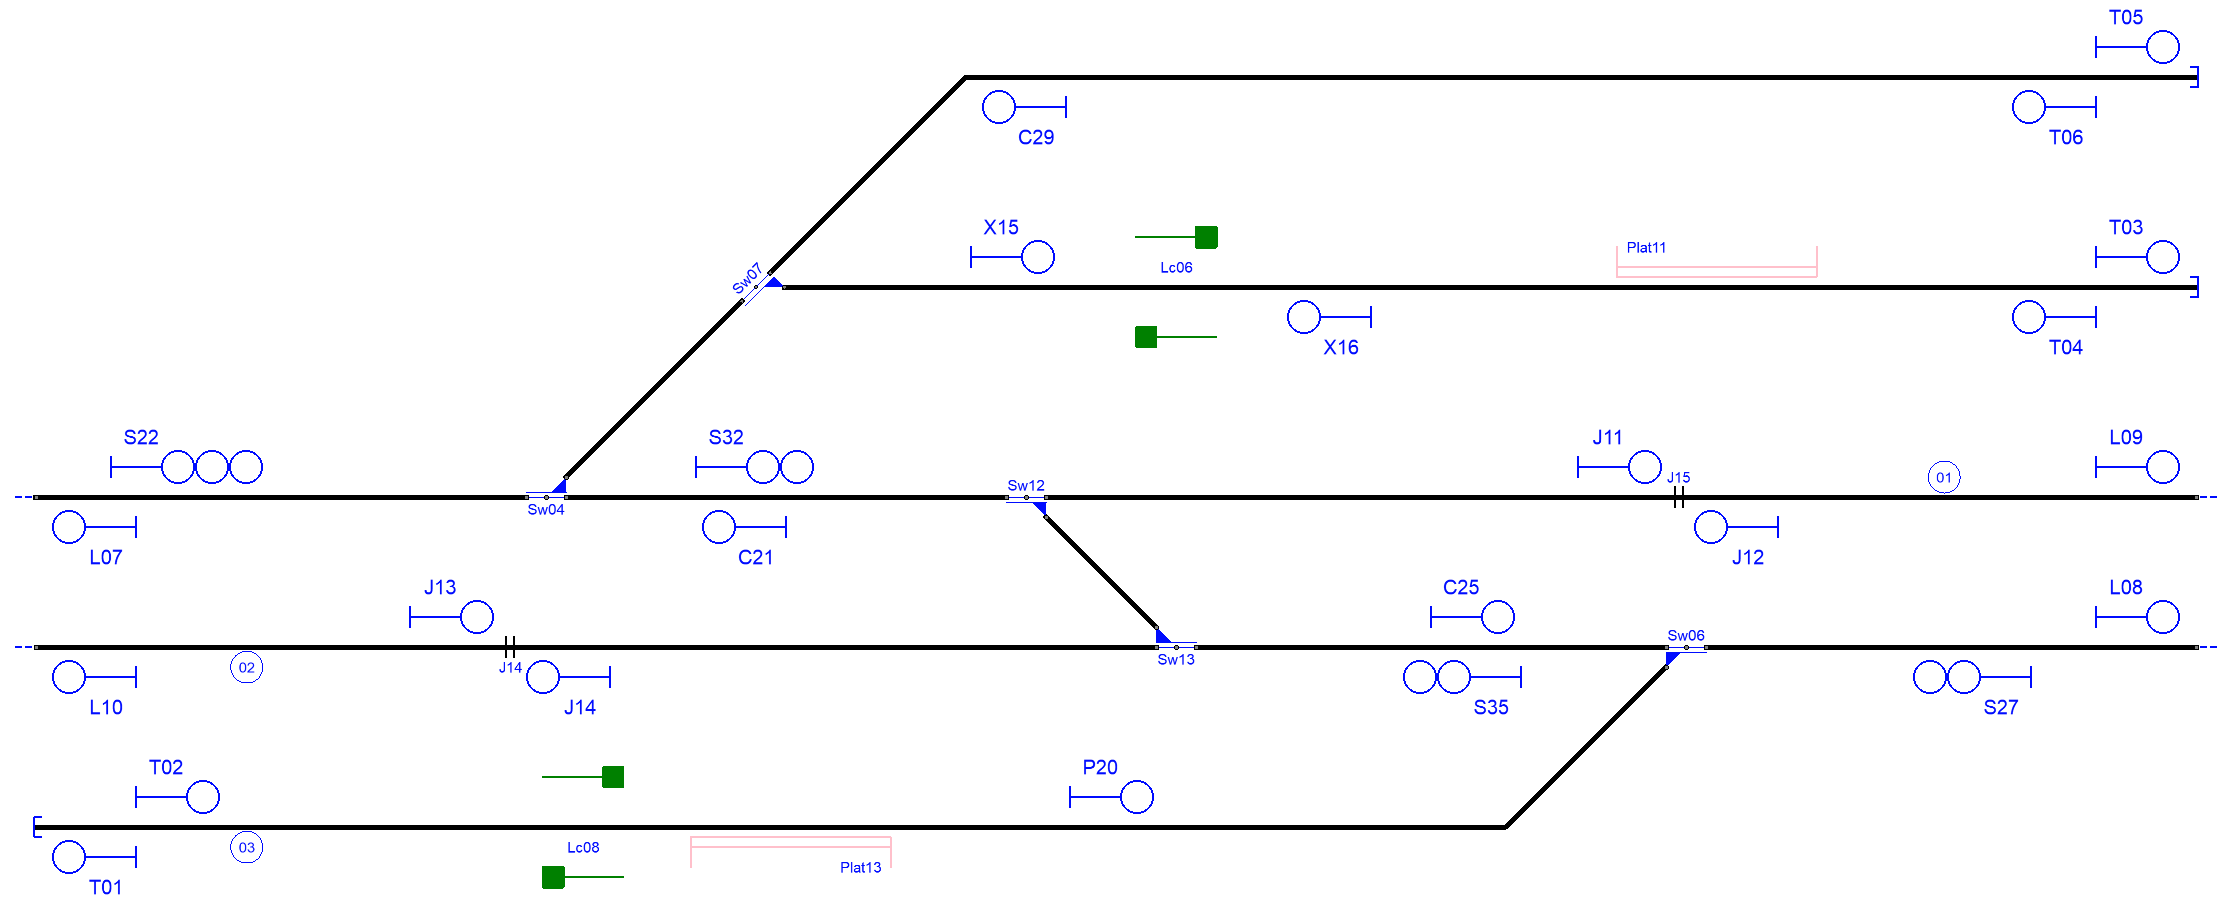
\includegraphics[width=1\textwidth]{resultados-obtenidos/ejemplo1/images/1_RNA.png}
        \centering\caption{Señalamiento generado y simplificado por el RNA.}
        %\label{fig:LC_P2}
    \end{figure}
    
    \lipsum[1]    
    
    \subsection{Señalamiento original}

    El señalamiento diseñado en forma manual por el autor de esta tesis para la topología de la Figura \ref{fig:EJ1_1} se ilustra en la Figura \ref{fig:EJ1_2}. Se observa que incluye señales de parada próximas a los finales de vías absolutos (S18, S19, S20), señales de partida en las plataformas (S04, S06, S08, S09), señales de protección antes de cada paso a nivel (S04, S05), señales de maniobras antes de converger en una vía principal (S03, S08) y señales múltiples para cambios de vías divergentes (S01, S17, S10, S07), entre varias otras señales. Estas señales permiten definir hasta un máximo de 14 rutas, todas ellas detalladas en la Tabla \ref{Tab:tabla_original_1}
    
    \begin{figure}[H]
    	\centering
    	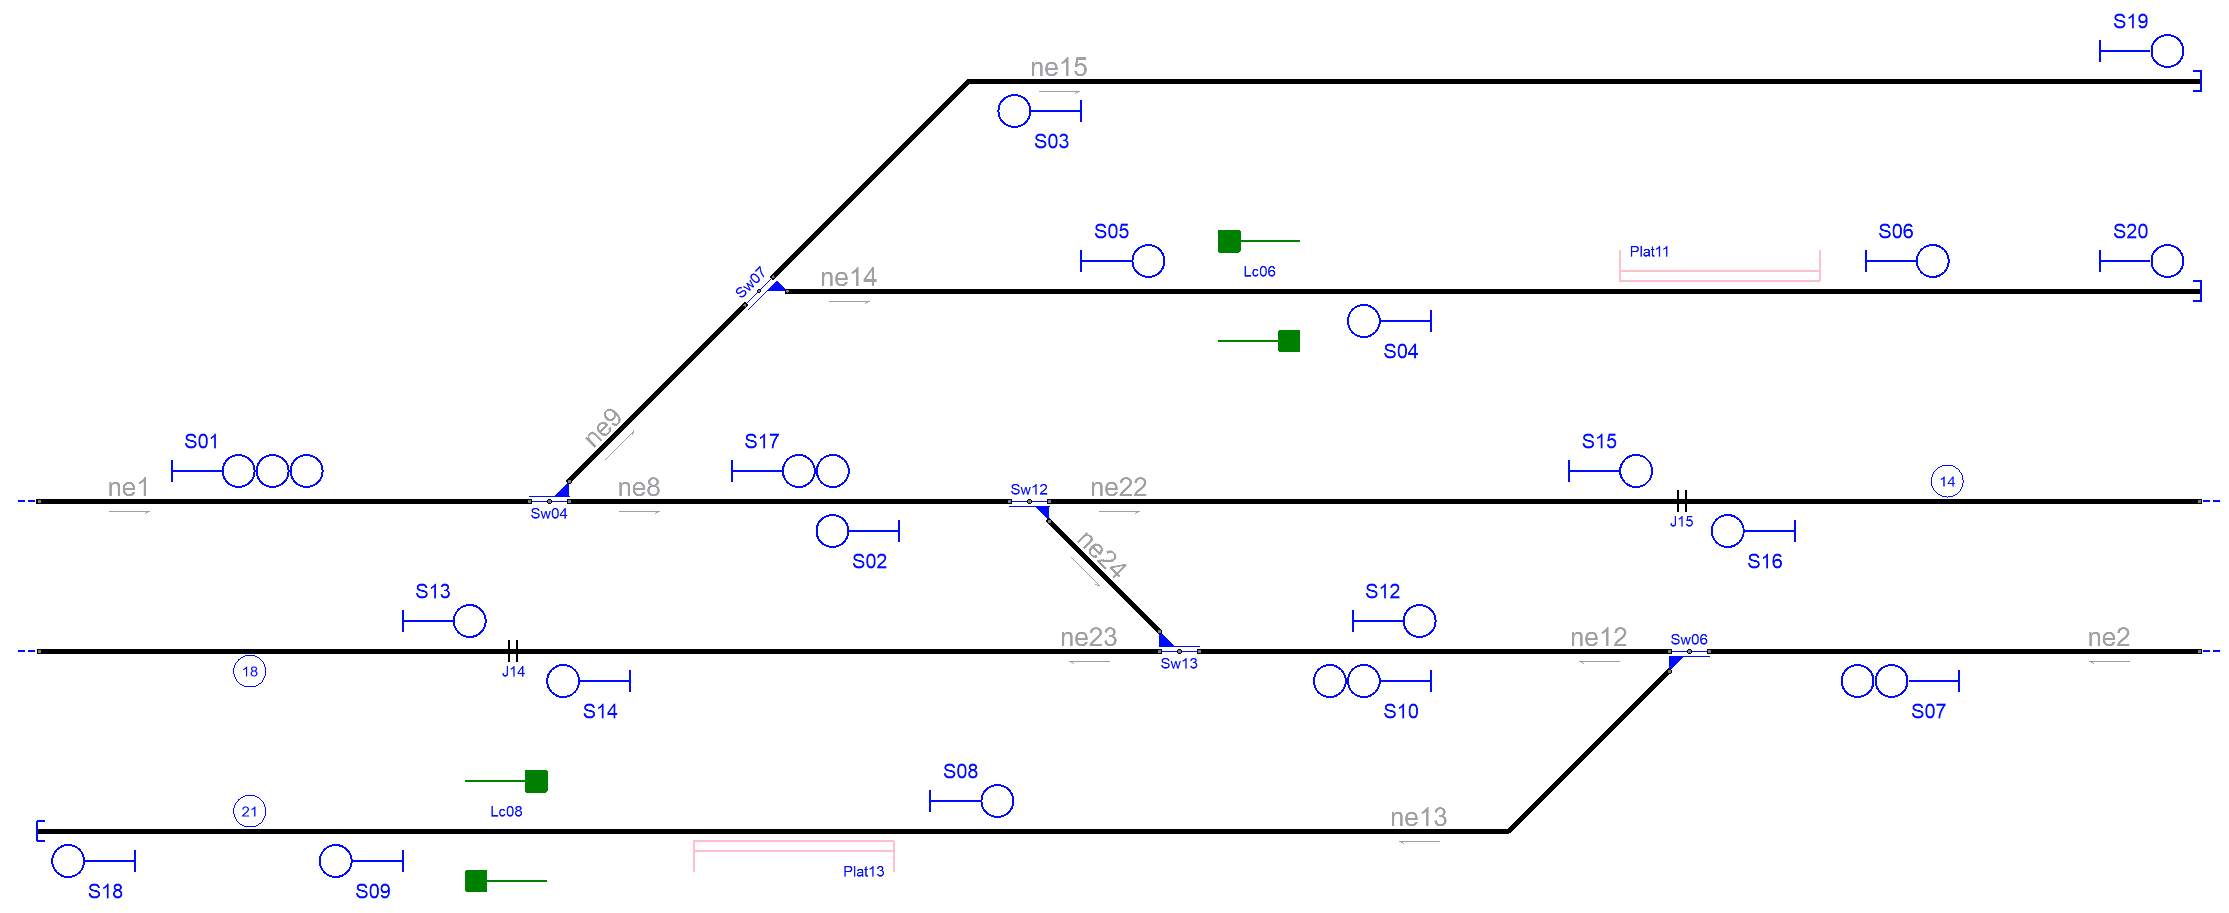
\includegraphics[width=1\textwidth]{resultados-obtenidos/ejemplo1/images/1_original.png}
    	\centering\caption{Señalamiento original del ejemplo 1.}
    	\label{fig:EJ1_2}
    \end{figure}
    
    En una primera inspección, se puede comprobar que todos los elementos ferroviarios son alcanzados por al menos una de las rutas, en al menos una dirección. Además, todos los cambios de vías son utilizados, de forma simple o compuesta. 
    
    \begin{table}[H]
        {
        \caption{Tabla de enclavamiento original del ejemplo 1.}
        \label{Tab:tabla_original_1}
        \centering
        \resizebox{1\textwidth}{!}{
            \begin{tabular}{ c c c c c c c }
                \hline	
                    Ruta & Inicio & Final & Cambio & Plataforma & Cruce & netElement \\	
                \hline
                    R$_{01}$  & S$_{05}$ & S$_{06}$ & - & Plat$_{11}$ & Lc$_{06}$ & ne$_{14}$\\
                    R$_{02}$  & S$_{06}$ & S$_{20}$ & - & - & - & ne$_{14}$\\
                    R$_{03}$  & S$_{09}$ & S$_{18}$ & - & - & - & ne$_{13}$\\
                    R$_{04}$  & S$_{13}$ & S$_{12}$ & Sw$_{13}^{N}$ & - & - & ne$_{23}$-ne$_{12}$\\
                    R$_{05}$  & S$_{16}$ & S$_{02}$ & Sw$_{12}^{N}$ & - & - & ne$_{22}$-ne$_{08}$\\
                    R$_{06}$  & S$_{07}$ & S$_{10}$ & Sw$_{06}^{N}$ & - & - & ne$_{02}$-ne$_{12}$\\
                    R$_{07}$  & S$_{07}$ & S$_{09}$ & Sw$_{06}^{R}$ & Plat$_{13}$ & Lc$_{08}$ & ne$_{02}$-ne$_{13}$\\
                    R$_{08}$  & S$_{10}$ & S$_{14}$ & Sw$_{13}^{N}$ & - & - & ne$_{12}$-ne$_{23}$\\
                    R$_{09}$  & S$_{10}$ & S$_{02}$ & Sw$_{12}^{R}$+Sw$_{13}^{R}$ & - & - & ne$_{12}$-ne$_{24}$-ne$_{08}$\\
                    R$_{10}$  & S$_{01}$ & S$_{17}$ & Sw$_{04}^{N}$ & - & - & ne$_{01}$-ne$_{08}$\\
                    R$_{11}$  & S$_{01}$ & S$_{19}$ & Sw$_{04}^{R}$+Sw$_{07}^{N}$ & - & - & ne$_{01}$-ne$_{15}$\\
                    R$_{12}$  & S$_{01}$ & S$_{05}$ & Sw$_{04}^{R}$+Sw$_{07}^{R}$ & - & - & ne$_{01}$-ne$_{14}$\\
                    R$_{13}$  & S$_{17}$ & S$_{15}$ & Sw$_{12}^{N}$ & - & - & ne$_{08}$-ne$_{22}$\\
                    R$_{14}$  & S$_{17}$ & S$_{12}$ & Sw$_{12}^{R}$+Sw$_{13}^{R}$ & - & - & ne$_{08}$-ne$_{24}$-ne$_{12}$\\    
                \hline
            \end{tabular}
        }
     }
    \end{table}
    
    Algunas rutas abarcan mas de un \textit{netElement}, como por ejemplo la ruta R14 que comienza en la señal S17 y finaliza en la señal S12, atraviesa los \textit{netElements} ne8, ne24 y ne12, y utiliza los cambios de vías Sw12 y Sw13, ambos en posición reversa.

    \subsection{Señalamiento generado por el RNA}

    \lipsum[1]
    
    \begin{table}[!h]
        {
        \caption{Tabla de enclavamiento del ejemplo 1 generada por el RNA.}
        \label{Tab:tabla_generated_1}
        \centering
        \resizebox{1\textwidth}{!}{
            \begin{tabular}{ c c c c c c c }
                \hline	
                    Ruta & Inicio & Final & Cambio & Plataforma & Cruce & netElement \\	
                \hline
                    R$_{01}$  & T$_{02}$ & P$_{20}$ & - & Plat$_{13}$ & Lc$_{08}$ & ne$_{13}$\\
                    R$_{02}$  & T$_{04}$ & X$_{16}$ & - & Plat$_{11}$ & - & ne$_{14}$\\
                    R$_{03}$  & T$_{06}$ & C$_{29}$ & - & - & - & ne$_{15}$\\
                    R$_{04}$  & J$_{11}$ & L$_{09}$ & - & - & - & ne$_{22}$\\
                    R$_{05}$  & J$_{12}$ & C$_{21}$ & Sw$_{12}^{N}$ & - & - & ne$_{22}$-ne$_{08}$\\
                    R$_{06}$  & J$_{13}$ & C$_{25}$ & Sw$_{13}^{N}$ & - & Lc$_{08}$ & ne$_{23}$-ne$_{12}$\\
                    R$_{07}$  & X$_{15}$ & T$_{03}$ & - & Plat$_{11}$ & Lc$_{06}$ & ne$_{14}$\\
                    R$_{08}$  & X$_{16}$ & L$_{07}$ & Sw$_{04}^{R}$+Sw$_{07}^{R}$ & - & - & ne$_{14}$-ne$_{01}$\\
                    R$_{09}$  & P$_{20}$ & L$_{08}$ & Sw$_{06}^{R}$ & - & - & ne$_{13}$-ne$_{02}$\\
                    R$_{10}$  & C$_{21}$ & L$_{07}$ & Sw$_{04}^{N}$ & - & - & ne$_{08}$-ne$_{01}$\\
                    R$_{11}$  & S$_{22}$ & S$_{32}$ & Sw$_{04}^{N}$ & - & - & ne$_{01}$-ne$_{08}$\\
                    R$_{12}$  & S$_{22}$ & X$_{15}$ & Sw$_{04}^{R}$+Sw$_{07}^{R}$ & - & - & ne$_{01}$-ne$_{14}$\\
                    R$_{13}$  & S$_{22}$ & T$_{05}$ & Sw$_{04}^{R}$+Sw$_{07}^{N}$ & - & - & ne$_{01}$-ne$_{15}$\\
                    R$_{14}$  & C$_{25}$ & L$_{08}$ & Sw$_{06}^{N}$ & - & - & ne$_{12}$-ne$_{02}$\\
                    R$_{15}$  & S$_{27}$ & S$_{35}$ & Sw$_{06}^{N}$ & - & - & ne$_{02}$-ne$_{12}$\\
                    R$_{16}$  & S$_{27}$ & T$_{01}$ & Sw$_{06}^{R}$ & Plat$_{13}$ & Lc$_{08}$ & ne$_{02}$-ne$_{13}$\\
                    R$_{17}$  & C$_{29}$ & L$_{07}$ & Sw$_{04}^{R}$+Sw$_{07}^{N}$ & - & - & ne$_{15}$-ne$_{01}$\\
                    R$_{18}$  & S$_{32}$ & J$_{11}$ & Sw$_{12}^{N}$ & - & - & ne$_{08}$-ne$_{22}$\\
                    R$_{19}$  & S$_{32}$ & C$_{25}$ & Sw$_{12}^{R}$+Sw$_{13}^{R}$ & - & - & ne$_{08}$-ne$_{12}$\\
                    R$_{20}$  & S$_{35}$ & J$_{14}$ & Sw$_{13}^{N}$ & - & - & ne$_{12}$-ne$_{23}$\\
                    R$_{21}$  & S$_{35}$ & C$_{21}$ & Sw$_{12}^{R}$+Sw$_{13}^{R}$ & - & - & ne$_{12}$-ne$_{08}$\\
                \hline
            \end{tabular}
        }
     }
    \end{table}
    \subsection{Sistema generado por el ACG}
	\label{sec:EJEMPLO1_ACG}
	
	En base a la red de grafos, ilustrada en la Figura \ref{fig:EJ1_8}, el ACG determinó la cantidad de elementos ferroviarios de cada tipo, tal como puede visualizarse en el Código \ref{lst:EJ1_8}.
	
	\begin{lstlisting}[language = {}, caption = Cantidad de elementos a implementar por el ACG, label = {lst:EJ1_8}]
	n_netElements:11
	n_switch:5
	n_doubleSwitch:0
	n_borders:4
	n_buffers:3
	n_levelCrossings:2
	n_platforms:2
	n_scissorCrossings:0
	n_signals:23
	N : 62
	\end{lstlisting}
	
	El ACG genera, en el caso de este ejemplo, 80 archivos en formato VHDL, tal como se puede visualizar en la Figura \ref{fig:EJ1_ACG_1}. Podemos destacar de la Figura \ref{fig:EJ1_ACG_1} al archivo \textit{Arty\_Z7-10.XDC}, que define los pines de entrada y salida de la plataforma Arty Z7 10 y Arty Z7 20. Este archivo es provisto por Xilinx para esta familia de plataformas. En caso de utilizar otra plataforma, se deberá incluir el archivo XDC correspondiente. En ambos casos, cada desarrollador debe asignar manualmente los pines a cada puerto del sistema generado por el ACG.
	
	\begin{figure}[H]
		\centering
		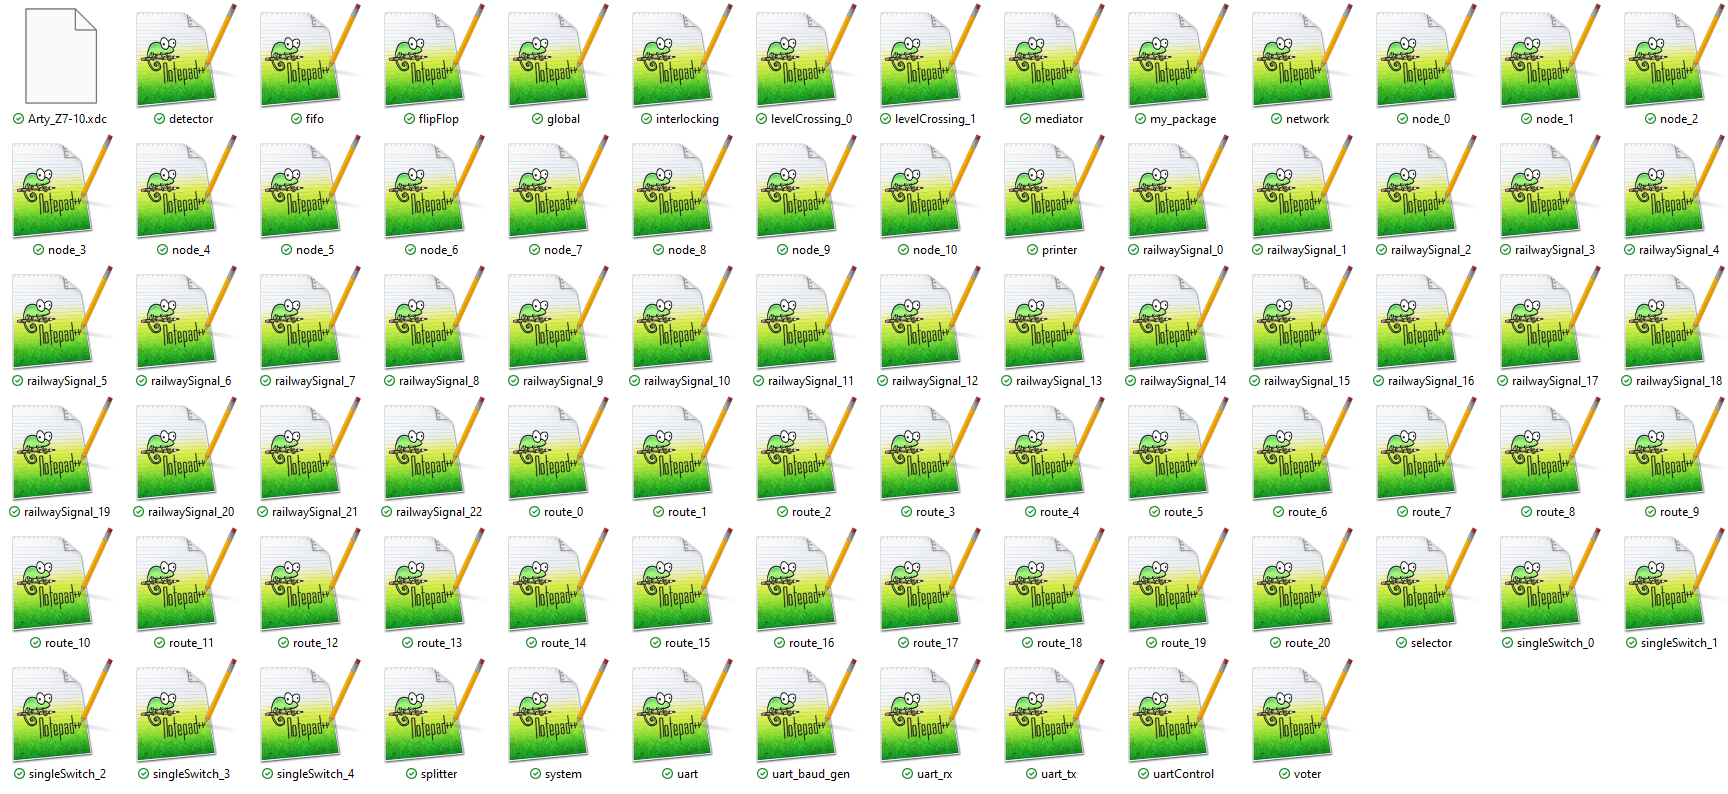
\includegraphics[origin = c, width=1\textwidth]{resultados-obtenidos/ejemplo1/images/ACG_files}
		\centering\caption{Archivos generador por el ACG para el ejemplo 1.}
		\label{fig:EJ1_ACG_1}
	\end{figure}
	
	Además, podemos mencionar los archivos \textit{my\_package.VHDL} y \textit{flipFlop.VHDL}, ambos generados por el ACG. El primero es una librería que define todos los tipos de datos utilizados por el sistema, y el segundo es un flip-flop tipo D utilizado para generar la secuencia de shift registers necesarios para adaptar el clock de entrada a los diferentes dominios de clock necesarios para el timeout de cada elemento ferroviario.
	
	Los archivos restantes son archivos que definen los módulos de alto nivel explicados en la Sección \ref{sec:interlockingArch} o la representación en VHDL de cada elemento ferroviario explicado entre la Sección \ref{sec:ACG_lc} y la Sección \ref{sec:ACG_rts}. Por ejemplo, en base lo descrito en el Código \ref{lst:EJ1_8}, hay 23 señales ferroviarias y podemos visualizar en la Figura \ref{fig:EJ1_ACG_1} 23 archivos referidos a las señales ferroviarias: desde \textit{railwaySignal\_0} hasta \textit{railwaySignal\_22}.
	
	Cada ejemplo cuenta con su propia carpeta de principio a fin. Es decir, el archivo railML original, los archivos generados por el RNA y el código generado por el ACG se encuentran en carpetas individuales para cada ejemplo. Esto es una ventaja a la hora de mantener un orden pero una gran desventaja a la hora de sintetizar los proyectos en Vivado. Cada conjunto de archivos debería ser importado de manera individual, previa desvinculación de los archivos del proyecto anterior. Para solucionar este inconveniente se desarrolló el Código \ref{lst:EJ1_script}, que automatiza la importación y desvinculación de los archivos de cada ejemplo.
	
	
	\begin{lstlisting}[language = {bash}, caption = script.tcl, label = {lst:EJ1_script}]
set chosen 1

# Get a list of all design source files
set design_sources [get_files -of_objects [get_filesets sources_1]]

remove_files $design_sources

set base_folder_path "ROOT/GICSAFePhD/App/Layouts/Example_"
set folder_path "${base_folder_path}${chosen}/VHDL"

puts $folder_path

set files [glob -directory $folder_path *.vhd]

add_files -norecurse -scan_for_includes  $files

update_compile_order -fileset sources_1
update_compile_order -fileset sources_1

synth_design -rtl -rtl_skip_mlo -name rtl_1
	\end{lstlisting}
	
	El parámetro \textit{chosen} indica el número de ejemplo seleccionado, mientras que \textit{base\_folder\_path} es la ruta absoluta de los ejemplos, cuyas carpetas deben ser nombradas como \textit{Example\_}+\textit{chosen} para poder ser encontradas. El Código \ref{lst:EJ1_script} puede ser importado en Vivado desde \textit{Tools $>$ Custom Commands $>$ Customize Commands} como un archivo TCL (del inglés, Tool Command Language), que es el formato que define los comandos nativos de Vivado. Pueden importarse tantos archivos TCL como se deseen, uno por cada ejemplo a sintetizar. De esta manera, cada script aparecerá en la barra de acceso rápido de Vivado de forma independiente y se automatiza el proceso de sincronización de archivos.
	
	Una vez ejecutado el script, Vivado ordenará los archivos de forma jerárquica, como puede verse en la parte izquierda de la Figura \ref{fig:EJ1_ACG_Vivado} donde el módulo \textit{global} incluye todos los módulos que fueron detallados en la Sección \ref{sec:interlockingArch}. Podemos destacar al módulo \textit{network} que es instanciado 3 veces junto con el módulo \textit{voter}, al ser una redundancia 2oo3, tal fue explicado en la Sección \ref{sec:VHDL2oo3}. Cada una de las instancias del módulo \textit{network} contienen sus propias 62 instancias de los mismos módulos de cada elemento ferroviario ya que N, cantidad de elementos ferroviarios, es 62 en el Código \ref{lst:EJ1_8}.	
	
	\begin{figure}[H]
		\centering
		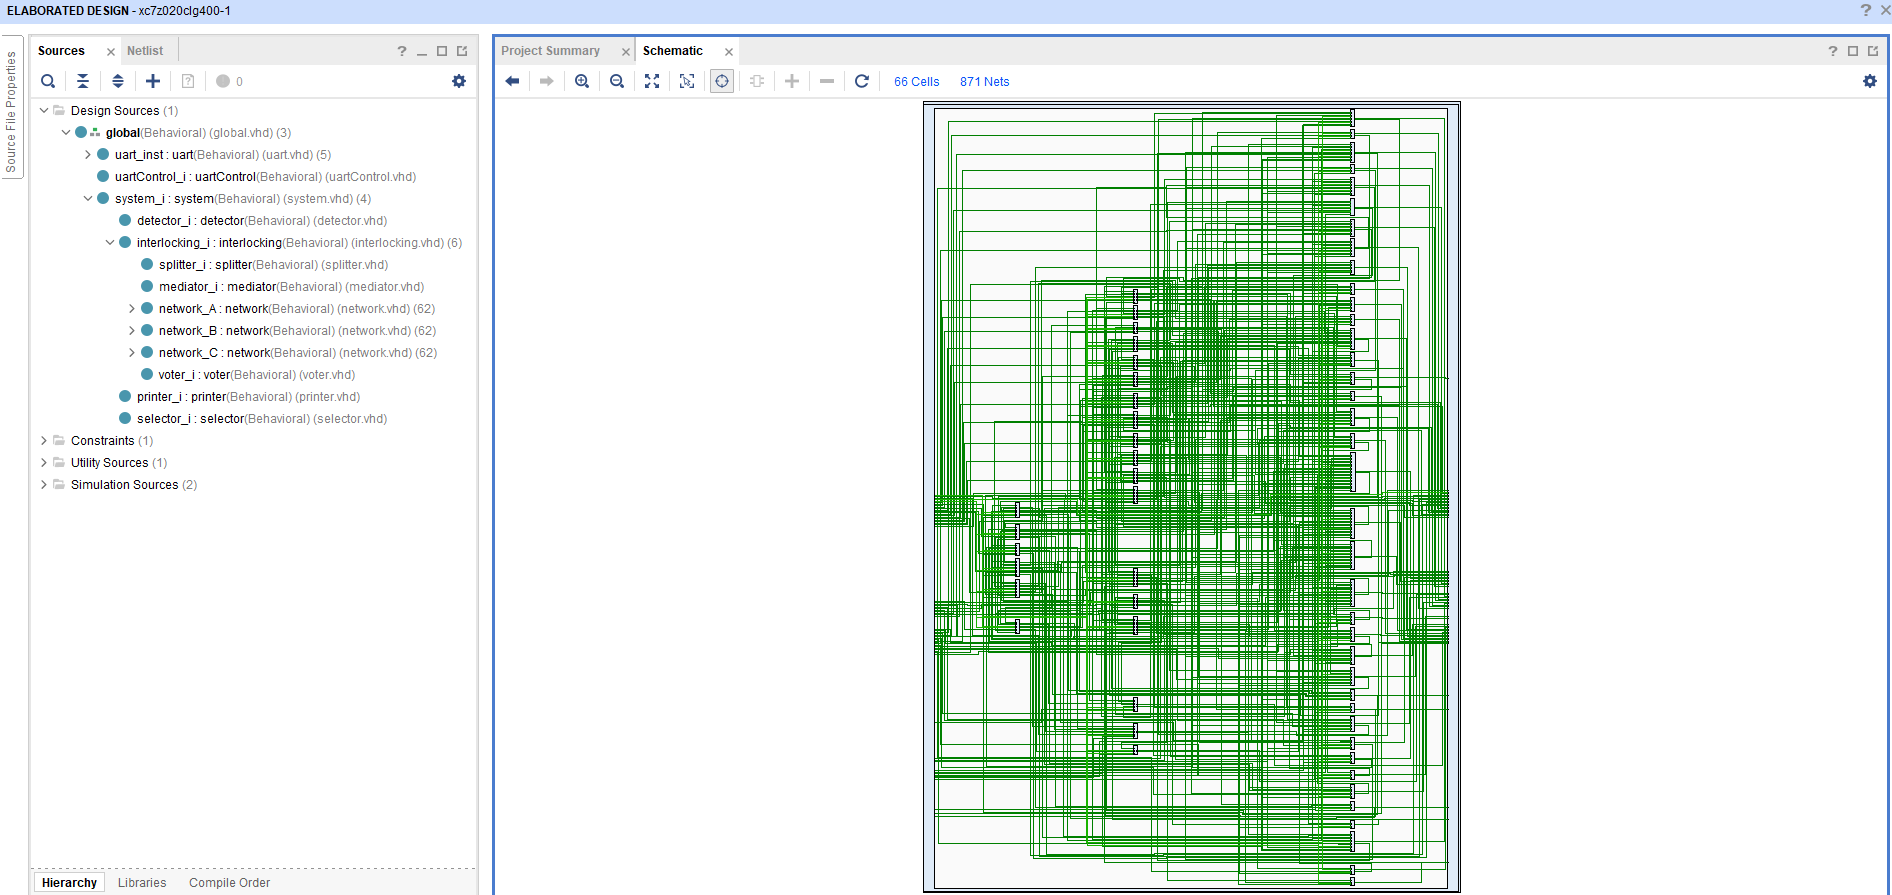
\includegraphics[origin = c, width=1\textwidth]{resultados-obtenidos/ejemplo1/images/ACG_vivado}
		\centering\caption{Interfaz del entorno de desarrollo Vivado para el ejemplo 1.}
		\label{fig:EJ1_ACG_Vivado}
	\end{figure}
	
	La parte derecha de la Figura \ref{fig:EJ1_ACG_Vivado} ilustra la representación en diagrama de bloques de uno de los módulos \textit{network} (los tres módulos tienen los mismos bloques). Puede apreciarse en esta ventana que existen 66 módulos interconectados de forma compleja utilizando 871 señales. Pero esto es solamente una porción del sistema generado por el ACG, de inspeccionar cada uno de los bloques es posible determinar que el ejemplo 1 utiliza 9517 sub módulos conectados automáticamente mediante 21899 señales, lo cual se aleja bastante de un desarrollo que pueda realizarse manualmente de forma trivial.
	
	Una vez que Vivado ha generado el diagrama de bloques ya tenemos la certeza de que el código VHDL ha pasado la prueba de sintaxis del entorno de desarrollo. A continuación, se deberá sintetizar e implementar el sistema para generar el bitstream que será utilizado para programar la FPGA. Durante el proceso de síntesis, Vivado busca la mejor forma de representar el código VHDL con compuertas lógicas, por lo que un código de mejor calidad brindará una representación en hardware lo mas fiel posible a lo buscado. Durante el proceso de implementación, en cambio, Vivado calcula si la representación con compuertas lógicas es posible de realizarse con la plataforma disponible. En este proceso influye no solamente la cantidad de compuertas disponibles sino también el tipo de compuertas. Si la plataforma no cuenta con la cantidad suficiente de compuertas A, entonces Vivado buscará la forma de reemplazar esa compuerta por otras compuertas B, C o D, que sean su equivalente lógico. Este proceso de reemplazo y/o simplificación puede llevar a que ambos procesos presenten discrepancias en la cantidad de elementos utilizados. 
	
	Los resultados de ambos procesos son detallados en la Tabla \ref{Tab:tabla_ACG_1}. Los porcentajes de uso son calculados por Vivado automáticamente, teniendo en cuenta que la plataforma Arty Z7 20 posee 53200 Look-Up-Tables (LUTs), 106400 Flip-Flops (FFs), 125 Pines de entrada y salida (IOs) y 32 Buffers (BUFGs), tal cómo se explicó en la Sección \ref{sec:AGG}. En este ejemplo, la cantidad de recursos utilizados es baja y el tiempo de síntesis e implementación es de 47 y 44 segundos, respectivamente.
	
	\begin{table}[H]
		{
			\caption{Síntesis e implementación del ejemplo 1 generado por el ACG.}
			\label{Tab:tabla_ACG_1}
			\centering
			%\small
			%\centering
			\begin{center}
				\resizebox{0.7\textwidth}{!}{
					\begin{tabular}{ c c c c }
						\hline	
						Recursos & Síntesis & Implementación & Uso \\	
						\hline
						LUT & 3457 & 3416 & 6.42/6.50\%\\
						FF & 3810 & 3813 & 3.58\%\\
						IO & 15 & 15 & 12.00\%\\
						BUFG & 3 & 3 & 9.38\%\\
						\hline
					\end{tabular}
				}
			\end{center}
		}    
	\end{table}
	
	
	
    \subsection{Validación del sistema de enclavamientos}

    Las 14 rutas del señalamiento original (Tabla \ref{Tab:tabla_original_1}) tienen 14 rutas equivalentes en el señalamiento generado por el RNA (Tabla \ref{Tab:tabla_generated_1}), tal como se puede visualizar en la Tabla \ref{Tab:tabla_validation_1}, generada automáticamente por el RNA.

    \begin{table}[H]
        {
        \caption{Equivalencias entre las rutas originales y las generadas por el RNA.}
        \label{Tab:tabla_validation_1}
        \centering
        %\small
            %\centering
            \begin{center}
            \resizebox{0.7\textwidth}{!}{
            \begin{tabular}{ c c c c }
                \hline	
                    Original & Señales & RNA & Señales \\	
                \hline
                    R$_{01}$ & S$_{05}$-S$_{06}$ & R$_{07}$ & X$_{15}$-T$_{03}$ \\
                    R$_{02}$ & S$_{06}$-S$_{20}$ & R$_{07}$ & X$_{15}$-T$_{03}$ \\
                    R$_{03}$ & S$_{09}$-S$_{18}$ & R$_{16}$ & S$_{27}$-T$_{01}$ \\
                    R$_{04}$ & S$_{13}$-S$_{12}$ & R$_{06}$ & J$_{13}$-C$_{25}$ \\
                    R$_{05}$ & S$_{16}$-S$_{02}$ & R$_{05}$ & J$_{12}$-C$_{21}$ \\
                    R$_{06}$ & S$_{07}$-S$_{10}$ & R$_{15}$ & S$_{27}$-S$_{35}$ \\
                    R$_{07}$ & S$_{07}$-S$_{09}$ & R$_{16}$ & S$_{27}$-T$_{01}$ \\
                    R$_{08}$ & S$_{10}$-S$_{14}$ & R$_{20}$ & S$_{35}$-J$_{14}$ \\
                    R$_{09}$ & S$_{10}$-S$_{02}$ & R$_{21}$ & S$_{35}$-C$_{21}$ \\
                    R$_{10}$ & S$_{01}$-S$_{17}$ & R$_{11}$ & S$_{22}$-S$_{32}$ \\
                    R$_{11}$ & S$_{01}$-S$_{19}$ & R$_{13}$ & S$_{22}$-X$_{15}$ \\
                    R$_{12}$ & S$_{01}$-S$_{05}$ & R$_{12}$ & S$_{22}$-T$_{05}$ \\
                    R$_{13}$ & S$_{17}$-S$_{15}$ & R$_{18}$ & S$_{32}$-J$_{11}$ \\
                    R$_{14}$ & S$_{17}$-S$_{12}$ & R$_{19}$ & S$_{32}$-C$_{25}$ \\   
                \hline
            \end{tabular}
            }
            \end{center}
        }    
    \end{table}
    
    Las rutas R1, R2, R3, R4, R7, R8, R9, R10, R13, R14 y R16 (Tabla \ref{Tab:tabla_generated_1}) generadas por el RNA que no tienen equivalencias en el señalamiento original (Tabla \ref{Tab:tabla_original_1}) se deben a que el RNA creó señales extras. Las señales T01, T02, T03, T04, T05 y T06 fueron creadas por el RNA para proteger los finales de vía absolutos, mientras que las señales L07, L08, L09 y L10 fueron creadas para proteger los finales de vías relativos. Estas nuevas señales constituyen nuevas rutas que permiten a las formaciones detenerse previo al final (relativo o absoluto) de la red ferroviaria, lo cual incrementa la seguridad y añade nuevas rutas en sentido contrario, mejorando la logística. Estos elementos ferroviarios no se encontraban protegidos en el señalamiento original.
    
    El señalamiento original carecía de señales protegiendo los finales de vía absolutos y relativos. No obstante, esto no se debe a un error en el diseño original, sino a que el diseño de señalamientos en la vida real se encuentra restringido por las necesidades particulares de cada locación, operador o leyes locales. Algunos operadores priorizarán tener rutas largas, dejando largas distancias sin señalamiento electrónico. Algunas normativas pueden indicar que la protección de ciertos elementos puede ser optativa. En el caso de los finales de vía pueden utilizarse señales lumínicas intermitentes que no son controladas por el señalamiento.
    
    En otros ejemplos el señalamiento original puede estar "incompleto", es decir, solo se consideraron las rutas en un sentido determinado, en base al uso que se le quería dar a ese señalamiento. El RNA, en cambio, siempre generará el señalamiento completo, que abarque la totalidad de la red ferroviaria ingresada, a menos que se seleccione la opción de señalamiento parcial, que respetará el sentido único de circulación que se defina en cada vía.    
    
    %TODO VALIDACION ALGORITMOS
    
    
    
    
    